	\documentclass[../pfc.tex]{subfiles}
	\usepackage{float}
	
	\begin{document}
	
Para la fase de análisis dentro de las metodologías ágiles no existen preceptos firmes a cumplir, pero dado que se valora mucho la comunicación y las relaciones interpersonales, se establece que debería haber una serie de reuniones previas al inicio de los sprints para que el equipo pueda obtener contexto del proyecto y del dominio del mismo, así como ir escribiendo las historias de usuario y rellenar y priorizar el product backlog. En estas reuniones idealmente asistirían tanto el product owner, el scrum master y el equipo, pero con el prodcut owner, el scrum master y aquel del equipo que mejor pueda ayudar a escribir las historias puede ser suficiente, recordemos que no se está estimando, simplemente se escuchan las necesidades del product owner y estas se traducen en funcionalidades y estas a su vez en requisitos mediante historias de usuario. \\

Para acometer el trabajo y dividirlo en trozos mas manejables en estos casos se suele recurrir a escribir historias épicas, que más tarde ya si pueden particionar el scrum master y el equipo para posteriormente remitirlas al product owner para que este exprese su conformidad o sus matices a las historias de usuario ya redactadas en piezas manejables y que priorice el prodcut backlog inicial, teniendo en cuenta que tras la estimación inicial puede haber algún reordenamiento para aprovechar mejor los tiempos del sprint. 

Una vez las historias tienen una forma más o menos fija, recordemos que uno de los fines del agilismo es responder al cambio y más al cambio en los requisitos, se hace una reunión de estimación de las mismas. Como ya se ha comentado existen varias maneras de estimar la complejidad que suponen las historias de usuario, casi todas basadas en variaciones del poker planning que se explicó anteriormente. 

En el momento de redactar las historias de usuario conviene que de algún modo alguien, típicamente el scrum master o el product owner, se encargue de recordar los grandes objetivos del proyecto. Estos objetivos son los objetivos claros, concisos y lo mas sencillos posibles que mueven al cliente a dar comienzo al proyecto. Todas las historias de usuario, asi como las acciones que se lleven a cabo, deben alinearse con estos objetivos.

Para llevar a cabo todo este proceso se llevaron a cabo varias reuniones con el personal de la AECC, se cruzaron correos con historias redactadas, se conversó vía Hangout, Skype, Whatsapp, etc se volvió a reunir las veces que hicieron falta, hasta que dicho personal, que en este caso hacía el papel de product owner,  se sintió lo suficientemente cómodo con el redactado inicial de las historias de usuario y su priorización, sabiendo que después estas podrían modificarse. 

 
-Por una parte de las reuniones mantenidas con el cliente, en este caso la AECC.

-Por otra parte del libro que utiliza la AECC llamado \textbf{MIS CUIDADOS, DIARIO DE SALUD DE UN SUPERVIVIENTE DE CANCER} y que se utiliza de manera general sobre enfermos de cáncer que han superado esta enfermedad y sobre otros que todavía la siguen padeciendo.\\\\
	

	\section{Explicación detallada de las funcionalidades de la aplicación}

Este sería el proceso donde algún miembro del equipo ganaría contexto por parte del product owner, al este describirle lo que quiere, vamos a pasar al redactado final de las necesidades que se expresaron, pues debido a la inexperiencia de los miembros de la AECC en el mundo de la movilidad el punto de partida del proyecto estaba mucho más alejado de aquí. Esto en el argot del agilismo se llama educar al cliente, y como siempre se basa en la comunicación, las relaciones interpersonales y en la confianza mutua.

\textbf{USO SIN REGISTRO}

En todo momento se debe poder usar la app sin hacer ningún tipo de registro previo. Solamente algunas funcionalidades especificas necesitarán del mismo. Para ello los datos serán almacenados en el dispositivo, sin perjuicio de que puedan una vez registrado ser compartidos en "la nube" y se carguen en varios dispositivos.\\

	\textbf{PRINCIPAL}
	
	Este será el punto de entrada habitual a la aplicación. salvo la primera vez que se ofrecerá la posibilidad de realizar un pequeño tutorial en la misma. Al entrar en la misma se obtiene un pequeño resumen con los eventos de todo tipo proximos en el día de hoy o un texto que nos informe de la ausencia de algún tipo de evento para el día de hoy.\\
	
	\textbf{PERSONAJES}
	
	Una pequeña lista de contactos importantes relacionados con la enfermedad, como puedan ser el oncólogo, el psicólogo, familiares de especial relevancia, etc.
	
	Como toda lista de contactos podrán añadirse, modificarse, borrarse y consultarse cada uno de los ítems que la componen de una manera sencilla, siguiendo los lineamientos del SO en cuestión.
	
	Por cuestiones de practicidad y simplicidad, si se añade un contacto o se modifica en esta parte, lo hará también en la app general de contactos del SO. Esto es así para que en cualquiera de las listas el usuario pueda encontrar al contacto que busque y no se sienta desorientado manejando varias listas de contactos en el dispositivo móvil. \\
	
	\textbf{CITAS}
	
	Es una funcionalidad para introducir citas médicas en un calendario. En las mismas se podrá añadir al profesional que nos atiende si es que se conoce. 
	Poco después de una cita se generará una notificación preguntando por la misma, en la que se preguntará si la cita ha generado nuevas citas, momento en que se pasará a la pantalla para crear una nueva cita, cambios en la medicación, yendo a la lista de medicamentos para añadir o cambiar la dosis de los mismos, 
	Lista de citas Nombre de la cita, fecha y hora.
	Desde el propio item de la lista se podran añadir medicamentos, personas, sintomas y/o pruebas, al pulsar sobre la opción correspondiente nos llevará al listado de estás opciones añadiendose así.
	
	Añadir cita, en esta pantalla se permite ver al pinchar sobre el propio item de la lista ,editar, o pulsando el botón añadir del final de la lista crear una nueva, 
	dentro de la cita (añadir) se podrán añadir ubicación, personajes, medicamentos, pruebas y sintomas y asignar una alarma personalizable con fecha y hora (avisar) con antelacion.
	se puede ver sin editar
	
	Deberíamos añadir duración?
	
	Valorar si deberiamos gestionar la repeticion de los eventos
	
	¿En la ubicación se podria comunicar con google maps?
	
	¿Deberiamos mostrar en el item de la cita si ya poseee personas, pruebas, sintomas o medicacion?

	\textbf{AVATAR}
	
	Editar el perfil, Foto, nombre, apellidos, edad, cumpleaños... (1 pantalla), ¿Grupo sanguineo y alergenos tampoco estaría mal pero es informacion de otro nivel LOPD?
	
	PROYECTO AMPLIACION (asignar un agente personalizado para poder atender de manera personalizada al paciente Superviviente)\\
	


	

	\textbf{HORARIO}

	Vista dia, mes, con las actividades, citas, ¿Cumpleaños, aniverssario de enfermedad...?  
	al pinchar en una hora, dia, se podrá añadir rutina o cita, iria a la correspondiente lista de creacion de una nueva (1 pantalla)
	
	Deberian aparecer las citas y rutinas ocupando el espacio destinado a la duracion de las mismas.
	
	Revisar esta página
	https://code.google.com/p/yadview/\\
	

	\textbf{RUTINA}
	Lista de rutinas, desde la propia vista se podrán añadir rutinas, al pulsar sobre la opción correspondiente nos llevará al listado de estás opciones añadiendose así.
	
	Se podra ordenar por fecha, asc y desc, duracion de la actividad asc y desc pero sobre todo se podrá ordenar por satisfaccion de la misma.
	
	Añadir rutina, , en esta pantalla se permite ver al pinchar sobre el propio item de la lista ,editar, o pulsando el botón añadir del final de la lista crear una nueva,
	Valorar si deberiamos gestionar la repeticion de los elementos					
	dentro de la rutina (añadir) se podrán añadir personajes y asignar una alarma personalizable (avisar) con antelacion, se puede ver sin editar(2 pantallas)
	con una hora de aviso, hora de empiece de la actividad. Duración de las misma en horas, satisfaccion de 0 a 10
	
	Dentro se va a valorar tambien la satisfacción personal que se produce al hacer esto, podrá ser de 0 a 10
	
	AMPLIACION DE PROYECTO: Poder variar los avisos para que se hagan de manera repetitiva, por ejemplo repetir de manera semanal los jueves al estilo TICK TICK, llamarlo actividades en vez de Rutina\\ 
	

	\textbf{CITAS}
	
	Lista de citas Nombre de la cita, fecha y hora.
	Desde el propio item de la lista se podran añadir medicamentos, personas, sintomas y/o pruebas, al pulsar sobre la opción correspondiente nos llevará al listado de estás opciones añadiendose así.
	
	Añadir cita, en esta pantalla se permite ver al pinchar sobre el propio item de la lista ,editar, o pulsando el botón añadir del final de la lista crear una nueva, 
	dentro de la cita (añadir) se podrán añadir ubicación, personajes, medicamentos, pruebas y sintomas y asignar una alarma personalizable con fecha y hora (avisar) con antelacion.
	se puede ver sin editar
	
	Deberíamos añadir duración?
	
	Valorar si deberiamos gestionar la repeticion de los eventos
	
	¿En la ubicación se podria comunicar con google maps?
	
	¿Deberiamos mostrar en el item de la cita si ya poseee personas, pruebas, sintomas o medicacion?
	
	PROYECTO AMPLIACION Poder exportar e importar a google maps, conectar la ubicacion con google maps para poder ir\\
	
	
	\textbf{MEDICACION}
	Lista de medicamentos, lista de los medicamentos que tengamos con el boton de añadir al final y en la barra la posibilidad de ordenar en principio por orden ascendente o descendente,
	al pinchar sobre el elemento se visualiza, en las opciones de cada elemento se puede añadir a la cita, editar y borrar (confirmacion para borrar)
	
	Añadir medicamento, , en esta pantalla se permite ver al pinchar sobre el propio item de la lista ,editar, o pulsando el botón añadir del final de la lista crear una nueva, 
	dentro del medicamento (añadir) se podrá asignar una foto personalizable, o bien hacerla o añadirla de la galeria, viene una por defecto
	nombre, descripcion, 
	una alarma personalizable que avisar con antelacion, fecha inicio, hora inicio, fecha fin, hora fin, repetir cada tantas horas, dias, semanas, (esto se valorará)

	REVISAR LA FUNCION DE ALARMA EN ANDROID http://developer.android.com/reference/android/app/AlarmManager.html
	boton guardar 
	se puede ver sin editar, 
	dentro de la edición y visionado se podra añadir a una cita
	Se puede añadir el numero de medicamentos al drawer (se estudiará)
	
	PROYECTO AMPLIACION Llevar el stock de lo que lleva consumido el paciente y generar alertas para cuando se le acabe, duplicar tratamiento, para ahorrar trabajo, opciones de dosis.\\
	
	
	
	
	
	\textbf{PRUEBAS}
	
	Lista de personajes que tengamos con el boton de añadir al final y en la barra la posibilidad de ordenar en principio por orden de fecha ascendente o descendente,
	al pinchar sobre el elemento se visualiza, 
	en las opciones de cada elemento se puede añadir a la cita, editar y borrar confirmacion para borrar
	
	Añadir prueba, , en esta pantalla se permite ver al pinchar sobre el propio item de la lista ,editar, o pulsando el botón añadir del final de la lista crear una nueva, 
	dentro de la prueba (añadir) se podrá asignar una foto personalizable, o bien hacerla o añadirla de la galeria, viene una por defecto
	nombre, descripcion,
	fecha y hora de la misma
	se puede ver sin editar, dentro de la edición y visionado se podra añadir a una cita por ejemplo visita al oncólogo
	Se puede añadir el numero al drawer
	
	PROYECTO AMPLIACION poder subir documentos tipo pdf para no depender de la fotografia solo, llevar estadísticas\\
	
	
	\textbf{SINTOMAS}
	
	Lista de síntomas que tengamos con el boton de añadir al final y en la barra la posibilidad de ordenar en principio por orden de fecha ascendente o descendente,
	al pinchar sobre el elemento se visualiza, 
	en las opciones de cada elemento se puede añadir a la cita, editar y borrar confirmacion para borrar
	
	Añadir sintoma, , en esta pantalla se permite ver al pinchar sobre el propio item de la lista ,editar, o pulsando el botón añadir del final de la lista crear una nueva, 
	dentro de la prueba (añadir) se podrá asignar una foto personalizable, o bien hacerla o añadirla de la galeria, viene una por defecto
	nombre, descripcion de los sintomas,
	fecha y hora de la misma
	se puede ver sin editar, dentro de la edición y visionado se podra añadir a una cita por ejemplo visita al oncólogo
	Se puede añadir el numero al drawer
	
	PROYECTO AMPLIACION poder subir documentos tipo pdf para no depender de la fotografia solo, llevar estadísticas, poder conectar con los centros de salud, hospitales, \\
	
	
	\textbf{RECURSOS}
	Dentro de los resursos aparece meditacion con musica relajante e instrucciones para ello
	consejos generales, de alimentacion, de vida, de salud...
	telefonos de interés generales (DEBEMOS DECIDIR SI SE PUEDEN PERSONALIZAR)
	Noticias (podemos añadir el blog de la AECC o la cuenta de twitter que no esta nada mal)
	
	
	\textbf{AJUSTES}
	Editar el perfil, 
	tamaño de letra, 	
	tono para alertas de citas y rutinas, 
	color del led de notificación, 
	posibilidad de feedback,
	quienes somos o motivaciones (¿? pantallas)\\\\

	
	\section{Documento de Análisis}
	
	Aunque utilizamos una metología ágil, hay puntos en los que no nos podemos separar de la metodología tradicional.
			
	Es difícil capturar todos los requisitos a partir de unas cuantas reuniones, para nuestro caso, pudimos contar con la ayuda del libro "Mis Cuidados, diario de salud para supervivientes de cáncer"
			
	Una de las ventajas de utilizar este primer tipo de metodología, es el de poder adaptar de una manera mucho más eficiente los recursos a las fechas y a los requisitos, y poder modificar estos requisitos de manera "ágil" debido al panorama cambiante que podemos tener de cara al cliente.
			
	\begin{figure}
		\centering
		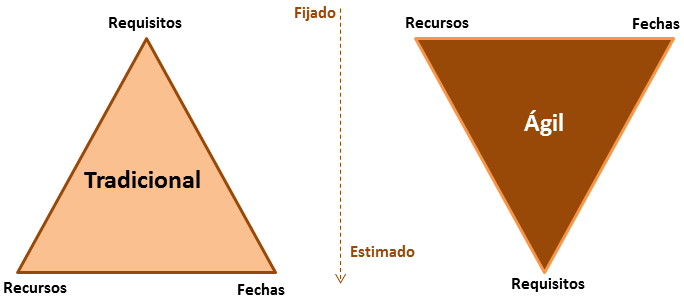
\includegraphics[width=0.5\linewidth]{../images/paradigmaRequisitos}
		\caption{Paradigma captura de requisitos método tradicional vs. ágil}
		\label{fig:paradigmaRequisitos}
	\end{figure}
			
			
	\subsection{Descripción de objetivos de manera detallada}
	
	
	\textbf{OBJ-001}	La aplicacion debera poder administrar un perfil de usuario\\*
	
		\begin{table}[H]
			\centering
			\begin{tabular}[t]{|l|l|}
				\hline \textbf{OBJ-001} & \textbf{PERFIL DE USUARIO} \\*
				\hline\hline \textbf{Versión} & 1.0 \\ *
				\hline\textbf{Autores} 	& Fernando Santa Olaya Rodríguez \\*
				& Rubén Toquero González\\*
				\hline \textbf{Descripción} & La aplicacion debera poder administrar un perfil de usuario\\* 
				\hline \textbf{Subobjetivos} & El usuario padrá introducir una foto, nombre, fecha de nacimiento \\* 
				\hline \textbf{Importacia} & Importante \\* 			
				\hline \textbf{Urgencia} & Inmediatamente \\* 
				\hline \textbf{Estado} & En construcción \\* 
				\hline \textbf{Estabilidad} & Estable \\* 
				\hline \textbf{Comentarios} & En la cabecera del drawer aparecerá el nombre y la foto \\* 
				\hline 
			\end{tabular}
			\caption{Menú drawer.}
			\label{tabla:req001}
		\end{table}
	
	\textbf{OBJ-002}	La aplicacion será facil de navegar para usuarios no avanzados\\*
	
	\textbf{OBJ-003}	La aplicacion facilitará la gestion de las actividades diarias de un usuario (medicas/rutinarias)\\*
	
	\textbf{OBJ-004}	La aplicacion permitirá gestionar de manera organizada las citas médicas de un usuario\\*
	
	\textbf{OBJ-005}	La aplicacion permitirá gestionar de manera organizada las rutinas diarias de un usuario\\*
	
	\textbf{OBJ-006}	La aplicacion permitirá gestionar de manera organizada los medicamentos asignados a un usuario\\*
	
	\textbf{OBJ-007}	La aplicacion permitirá gestionar de manera organizada los personajes que interactuan en las
	 actividades de un usuario\\*
	
	\textbf{OBJ-008}La aplicacion permitirá gestionar de manera organizada los síntomas que acontecen a un usuario\\*
	
	\textbf{OBJ-009}	La aplicacion permitirá gestionar de manera organizada las pruebas médicas a las que se somete un
	 usuario\\*
	
	\textbf{OBJ-010}	La aplicacion proporcionará recursos de ayuda para el bienestar del usuario\\*
	
	\textbf{OBJ-011}	La aplicación permitirá ajustes que mejoren la experiencia del usuario\\*
	
	\textbf{OBJ-012}	La aplicación deberá tener una base de datos para almacenar toda la informacion del usuario\\*
	
	\textbf{OBJ-013}	La aplicación deberá contar con un manual de usuario para facilitar su comprension y uso\\*
	
	\textbf{OBJ-014}	La aplicación soportará el mayor número de dispositivos android posibles\\*
	
	\textbf{OBJ-015}	La aplicación será de verdadera ayuda para usuarios incluidos dentro de la iniciativa de la AECC\\*
	
	\textbf{OBJ-016}	La aplicación se integrará perfectamente dentro de la iniciativa de la AECC\\*
	
	

	
	
	\subsection{Captura de Requisitos}
	
	Como consecuencia de las diferentes reuniones realizadas con el cliente se elabora un
	documento de especificación de requisitos con el propósito de describir las funcionalidades
	necesarias para poder validar el producto final.\\*
	
	\subsubsection{Requisitos de información}
			
	
	\subsubsection{Requisitos Funcionales}
	
	A continuación se describirán los requisitos para este proyecto. Se tendrán dos tipos de
	requisitos: requisitos funcionales, que serán aquellos obtenidos a partir de los objetivos principales
	y secundarios del apartado anterior; y requisitos no funcionales, obtenidos de las especificaciones
	citadas a lo largo de la memoria y que precisen ser descritas como requisitos.\\*
	
	Este tipo de requisitos declaran los servicios que debe proporcionar la aplicación, como debe
	reaccionar a una entrada particular y cómo se debe de comportar ante situaciones particulares.
	Describen el funcionamiento dla aplicación.\\*
	
	Los requisitos de información llevarán un nombre descriptivo y un número para identificarlos.
	Este número tendrá el formato IRQ - <id> donde id será el número del requisito de información.
	Además se indicarán los requisitos asociados, una descripción y cualquier información que sea
	relevante para una mayor claridad.\\*
	
	Los requisitos funcionales que debe cumplir la aplicación son los siguientes\\*
	
	
	\textbf{FRQ-001}	El usuario podra acceder a un menú de navegación	\textbf{OBJ-002}\\*

	\begin{table}[H]
		\centering
		\begin{tabular}[t]{|l|l|}
			\hline \textbf{FRQ-001} & \textbf{DRAWER MENÚ} \\*
			\hline\hline \textbf{Versión} & 1.0 \\ *
			\hline\textbf{Autores} 	& Fernando Santa Olaya Rodríguez\\*
			& Rubén Toquero González\\*
			\hline \textbf{Dependencias} & OBJ-002\\* 			
			\hline \textbf{Descripción} & El usuario podrá acceder a un menú de navegación \\* 
			\hline \textbf{Importancia} & Vital \\* 
			\hline \textbf{Urgencia} & Inmediatamente \\* 
			\hline \textbf{Estado} & En construcción \\* 
			\hline \textbf{Estabilidad} & Estable \\* 
			\hline \textbf{Comentarios} & El menú será visible al desplazar el dedo de izquierda a derecha de la pantalla \\* 
			\hline 
		\end{tabular}
		\caption{Menú drawer.}
		\label{tabla:req001}
	\end{table}
	
	
	\textbf{FRQ-002}	El usuario podrá introducir sus datos personales en la aplicación 	\textbf{OBJ-001}
	
	\textbf{FRQ-003}	El usuario podra visualizar sus datos personales	\textbf{OBJ-001}
	
	\textbf{FRQ-004}	Es usuario podrá ver/editar sus datos personales	\textbf{OBJ-001}\\*
	
	
	
	\textbf{FRQ-005}	El usuario al acceder a la aplicación podra visualizar de un vistazo su actividad para hoy 		\textbf{OBJ-003}
	
	\textbf{FRQ-006}	El usuario podrá acceder desde la pantalla principal a sus citas medicas	\textbf{OBJ-003 OBJ-004}
	
	\textbf{FRQ-007}	El usuario podrá acceder desde la pantalla principal a sus rutinas diarias	\textbf{OBJ-003}  \textbf{OBJ-005}\\*					
	
	
	AFECTADAS POR EL OBJETIVO \textbf{OBJ-004}\\*
	\textbf{FRQ-008}	La aplicación mostrará una vista del dia actual con actividades del usuario de ese dia (citas y rutinas)
	
	\textbf{FRQ-009}	La aplicación mostrará una vista del mes actual para las actividades del usuario de ese mes (citas y rutinas)	\textbf{OBJ-003}
	
	\textbf{FRQ-010}	El usuario podrá añadir una cita desde cualquiera de las vistas mensual/diaria
	
	\textbf{FRQ-011}	El usuario podrá añadir una rutina para ese dia desde cualquiera de las vistas mensual/diaria
	
	\textbf{FRQ-012}	El usuario podrá visualizar/editar la cita desde cualquiera de esas vistas
	
	\textbf{FRQ-013}	El usuario podrá visualizar/editar la rutina desde cualquiera de esas vistas\\*
	
	
	AFECTADOS POR EL OBJETIVO 	\textbf{OBJ-004}\\*
	
	\textbf{FRQ-014}	El usuario podrá acceder a la lista de citas medicas
	
	\textbf{FRQ-015}	El usuario podrá añadir desde la lista una nueva cita medica
	
	\textbf{FRQ-016}	El usuario podrá añadir alertas y notificaciones a una cita médica
	
	\textbf{FRQ-017}	El usuario podrá añadir personajes a una cita medica
	
	\textbf{FRQ-018}	El usuario podrá añadir pruebas a una cita medica
	
	\textbf{FRQ-019}	El usuario podrá añadir medicamentos a una cita medica
	
	\textbf{FRQ-020}	El usuario podrá añadir duración a una cita médica
	
	\textbf{FRQ-021}	El usuario podrá añadir síntomas a una cita medica
	
	\textbf{FRQ-022}	El usuario podrá visualizar/editar la cita medica\\*
	
	
	
	AFECTADOS POR EL OBJETIVO 	\textbf{OBJ-005}\\*
	\textbf{FRQ-023}	El usuario podrá acceder a la lista de rutinas
	
	\textbf{FRQ-024}	El usuario podrá añadir desde la lista una nueva rutina
	
	\textbf{FRQ-025}	El usuario podrá añadir alertas y notificaciones a una rutina
	
	\textbf{FRQ-026}	El usuario podrá añadir duración a una rutina
	
	\textbf{FRQ-027}	El usuario podrá añadir personajes a una rutina
	
	\textbf{FRQ-028}	El usuario podrá visualizar/editar la rutina\\*
	
	
	
	
	AFECTADOS POR EL OBJETIVO 	\textbf{OBJ-006}\\*
	\textbf{FRQ-029}	El usuario podrá acceder a la lista de medicamentos
	
	\textbf{FRQ-030}	El usuario podrá añadir desde la lista un nuevo medicamento
	
	\textbf{FRQ-031}	El usuario podra añadir información importante respecto a ese medicamento
	
	\textbf{FRQ-032}	El usuario podrá añadir alertas y notificaciones a medicamento
	
	\textbf{FRQ-033}	El usuario podrá visualizar/editar el medicamento\\*
	
	
	AFECTADOS POR EL OBJETIVO 	\textbf{OBJ-007}
	
	\textbf{FRQ-034 A FRQ-049}	Lo mismo con personajes, sintomas, pruebas\\*
	
	
	
	AFECTADOS POR EL OBJETIVO 	\textbf{OBJ-010}\\*
	\textbf{FRQ-050}	El usuario podrá acceder a recursos relaccionados con el autocontrol y la meditacion
	
	\textbf{FRQ-051}	El usuario tendrá acceso a telefonos de interés
	
	\textbf{FRQ-052}	El usuario tendrá acceso a consejos que le proporcionen bienestar
	
	\textbf{FRQ-053}	El usuario tendrá acceso a noticias relativas a la AECC\\*
	
	
	
	\textbf{FRQ-054}	La aplicación notificará al paciente a peticion citas y rutinas\\*
	
	\textbf{FRQ-055}	Las listas seran ordenable segun diferentes criterios\\*
	
	
	AFECTADOS POR EL OBJETIVO 	\textbf{OBJ-011}\\*
	\textbf{FRQ-056}	La aplicacion contendrá ajustes que faciliten su manejo al usuario\\*
	
	

	\subsubsection{Requisitos No Funcionales}
	
	Este tipo de requisitos define las propiedades emergentes dla aplicación, tales como el tiempo de
	respuesta, las necesidades de almacenamiento, la fiabilidad.\\*
	
	Pueden especificar también la utilización de una herramienta CASE en particular, un lenguaje
	de programación o un método del desarrollo.\\*
	
	En este apartado se detalla el catálogo de requisitos no funcionales. Estos requisitos pueden
	ser más críticos que los requisitos funcionales, ya que son a los que normalmente debe apuntar la
	arquitectura y si estos no son cumplidos, el software puede no funcionar o el cliente simplemente
	no acepta el producto.\\*
	
	Estos requisitos se puede decir que no están relacionados directamente con la funcionalidad
	dla aplicación. Con esto no se pretende decir que no sean necesarios para la funcionalidad dla aplicación,
	pero sí que no pueden asociarse a ningún caso de uso en particular. Hay distintas categorías y tipos
	de requisitos no funcionales: hardware, plataforma software, comunicaciones, de interfaz, de
	seguridad, de control de concurrencia, de persistencia…etc.\\*
	
	Los requisitos no funcionales llevarán un nombre descriptivo y un número para identificarlos.
	Este número tendrá el formato NFRQ - <id> donde id será el número del requisito de información.
	Además se indicará una descripción y cualquier información que sea relevante para una mayor
	claridad.\\*
	
	Algunos requisitos no funcionales identificados para el desarrollo del presente proyecto son
	los siguientes:\\*

	AFECTADOS POR EL OBJETIVO 	\textbf{OBJ-015}\\*
		
	\textbf{NFRQ-001}		La aplicacion será un apoyo y una ayuda para el paciente\\*
	
	
	AFECTADOS POR EL OBJETIVO 	\textbf{OBJ-016}\\*
		
	\textbf{NFRQ-002}		La aplicación debe ser coherente con el programa de Diario de Salud de la AECC.
	
	
	AFECTADOS POR EL OBJETIVO 	\textbf{OBJ-013 OBJ-015}\\*		
	\textbf{NFRQ-003}		La aplicacion sera amigable para usuarios no avanzados
	
	
	AFECTADOS POR EL OBJETIVO 	\textbf{OBJ-016}\\*	
	\textbf{NFRQ-004}		La aplicacion cumplira las guias de estilo fijadas por la AECC
	
	
	AFECTADOS POR EL OBJETIVO 	\textbf{OBJ-015}\\*		
	\textbf{NFRQ-005}		La aplicación proporcionará recursos de valor para los enfermos de cancer.
	
	
		
	\textbf{NFRQ-006}		La aplicación será mantenible y escalable a petición del cliente.


	AFECTADOS POR EL OBJETIVO 	\textbf{OBJ-004}\\*	
	\textbf{NFRQ-007}		La aplicación facilitara las visitas médicas


	AFECTADOS POR EL OBJETIVO 	\textbf{OBJ-005}\\*			
	\textbf{NFRQ-008}		La aplicacion incentivará la realizacion de actividades placenteras para el paciente


	AFECTADOS POR EL OBJETIVO 	\textbf{OBJ-003}\\*		
	\textbf{NFRQ-009}		La aplicacion facilitara la organizacion de los compromisos del usuario


		
	\textbf{NFRQ-010}		La aplicación será segura y confiable
	
	
	\textbf{NFRQ-011}		La aplicación estará finalizada antes del dia 9 de septiembre

	

	\subsection{Identificación de actores}
		
	\subsection{Diagrama de casos de uso }
		



	\subsection{Descripción de Casos de Uso}
	
	\textbf{CASOS DE USO}\\*
	
		
	\textbf{CU-001} PERFIL DE USUARIO - Inserción de perfil\\*
	
	\begin{table}[H]
		\centering
		\begin{tabular}[t]{|p{3cm}|p{9.5cm}|}
				\hline \textbf{CU-001} & \textbf{PERFIL DE USUARIO- INSERCIÓN} \\*
				\hline\hline \textbf{Versión} & 1.0 \\ *
				\hline\hline \textbf{Fecha} & 23/07/2015 \\ *
				\hline\textbf{Actores} 	& Usuario\\*
				\hline \textbf{Objetivo} & Incluir en la aplicación los datos personales del usuario\\* 			
				\hline \textbf{Precondición} & Los datos del usuario están sin completar \\* 
				\hline \textbf{Flujo normal} & 1.- Desplegamos el menú drawer \\* 
											 & 2.- Pulsamos el circulo que está al principio del menú \\*	
											 & 3.- Rellenamos los datos personales del usuario\\*	
				\hline \textbf{Flujo alternativo} & 1.- Desplegamos el menú drawer \\* 
 												  & 2.- Pulsamos la opcion ajustes \\*	
												  & 3.- Pulsamos la opción en pantalla "Perfil" \\*	
												  & 3.- Rellenamos los datos personales del usuario \\*	
				\hline \textbf{Postcondición} & El usuario posee sus datos personales en la aplicación \\* 
				\hline \textbf{Comentarios}   & A la hora de introducir la fotografía dentro de los datos personales, podrá elegir entre las que tenga en la galeria del propio terminal o acceder a la aplicación de cámara para hacer una nueva fotografía\\*
				\hline
			\end{tabular}
			\caption{Prefil de usuario - Inserción}
			\label{tabla:caso001}
	\end{table}
	
	
	
	\textbf{CU-002}	PERFIL DE USUARIO - Consulta de perfil\\*
	
	La visualización del perfil pude ser un caso de uso que converge con el anterior, comparten pre y post condición, y el flujo de acceso es prácticamente el mismo (Se estudiará)\\*
	
	\begin{table}[H]
		\centering
		\begin{tabular}[t]{|p{3cm}|p{9.5cm}|}
			\hline \textbf{CU-002} & \textbf{PERFIL DE USUARIO - CONSULTA} \\*
			\hline\hline \textbf{Versión} & 1.0 \\ *
			\hline\hline \textbf{Fecha} & 24/07/2015 \\ *
			\hline\textbf{Actores} 	& Usuario\\*
			\hline \textbf{Objetivo} & Consultar en la aplicación los datos personales del usuario\\* 			
			\hline \textbf{Precondición} & Los datos del usuario existen en la aplicación \\* 
			\hline \textbf{Flujo normal} & 1.- Desplegamos el menú drawer \\* 
			& 2.- Pulsamos el circulo que está al principio del menú \\*	
			& 3.- Consultamos los datos personales del usuario\\*	
			\hline \textbf{Flujo alternativo} & 1.- Desplegamos el menú drawer \\* 
			& 2.- Pulsamos la opción ajustes \\*	
			& 3.- Pulsamos la opción en pantalla "Perfil" \\*	
			& 3.- Rellenamos los datos personales del usuario \\*	
			\hline \textbf{Postcondición} & El usuario ha consultado sus datos personales\\* 
			\hline \textbf{Comentarios}   & Se pueden añadir aquí datos relativos a los campos que pueden existir en el perfil\\*
			\hline
		\end{tabular}
		\caption{Perfil de usuario - Consulta}
		\label{tabla:caso002}
	\end{table}
	
		
	\textbf{CU-003} PERFIL DE USUARIO - Edición de perfil\\*
	
	\begin{table}[H]
		\centering
		\begin{tabular}[t]{|p{3cm}|p{9.5cm}|}
			\hline \textbf{CU-003} & \textbf{PERFIL DE USUARIO - EDICIÓN} \\*
			\hline\hline \textbf{Versión} & 1.0 \\ *
			\hline\hline \textbf{Fecha} & 24/07/2015 \\ *
			\hline\textbf{Actores} 	& Usuario\\*
			\hline \textbf{Objetivo} & Modificar en la aplicación los datos personales del usuario\\* 			
			\hline \textbf{Precondición} & Los datos del usuario existen en la aplicación \\* 
			\hline \textbf{Flujo normal} & 1.- Desplegamos el menú drawer \\* 
			& 2.- Pulsamos el circulo que está al principio del menú \\*	
			& 3.- Rellenamos los datos personales del usuario\\*	
			\hline \textbf{Flujo alternativo} & 1.- Desplegamos el menú drawer \\* 
			& 2.- Pulsamos la opción ajustes \\*	
			& 3.- Pulsamos la opción en pantalla "Perfil" \\*	
			& 3.- Rellenamos los datos personales del usuario \\*	
			\hline \textbf{Postcondición} & El usuario posee sus datos personales modificados\\* 
			\hline \textbf{Comentarios}   & El usuario puede a su elección dejar los datos tal y como estuviesen en un principio\\*
			\hline
		\end{tabular}
		\caption{Perfil de usuario - Edición}
		\label{tabla:caso003}
	\end{table}
	
	
		
	\textbf{CU-004}	PERFIL DE USUARIO - Borrado de perfil\\*

	\begin{table}[H]
		\centering
		\begin{tabular}[t]{|p{3cm}|p{9.5cm}|}
			\hline \textbf{CU-004} & \textbf{PERFIL DE USUARIO - BORRADO} \\*
			\hline\hline \textbf{Versión} & 1.0 \\ *
			\hline\hline \textbf{Fecha} & 24/07/2015 \\ *
			\hline\textbf{Actores} 	& Usuario\\*
			\hline \textbf{Objetivo} & Borrar dla aplicación los datos personales del usuario\\* 			
			\hline \textbf{Precondición} & Los datos del usuario existen en la aplicación \\* 
			\hline \textbf{Flujo normal} & 1.- Desplegamos el menú drawer \\* 
			& 2.- Pulsamos el circulo que está al principio del menú \\*	
			& 3.- Rellenamos los datos personales del usuario\\*	
			\hline \textbf{Flujo alternativo} & 1.- Desplegamos el menú drawer \\* 
			& 2.- Pulsamos la opcion ajustes \\*	
			& 3.- Pulsamos la opción en pantalla "Perfil" \\*	
			& 3.- Rellenamos los datos personales del usuario \\*	
			\hline \textbf{Postcondición} & El usuario ya NO posee sus datos personales en la aplicación \\* 
			\hline \textbf{Comentarios}   &  \\*
			\hline
		\end{tabular}
		\caption{Perfil de usuario - Borrado}
		\label{tabla:caso004}
	\end{table}
	
	
	
	
	
	
	\textbf{CITA MEDICA}\\*

	\textbf{CU-005}	CITA MEDICA - Inserción de cita médica\\*
	
	\begin{table}[H]
		\centering
		\begin{tabular}[t]{|p{3cm}|p{9.5cm}|}
			\hline \textbf{CU-005} & \textbf{CITA MÉDICA - INSERCIÓN} \\*
			\hline\hline \textbf{Versión} & 1.0 \\ *
			\hline\hline \textbf{Fecha} & 27/07/2015 \\ *
			\hline\textbf{Actores} 	& Usuario\\*
			\hline \textbf{Objetivo} & Insertar en la aplicación una cita médica que tiene el usuario\\* 			
			\hline \textbf{Precondición} & La cita médica no existe en la aplicación\\* 
			\hline \textbf{Flujo normal} & 1.- Desplegamos el menú drawer \\* 
			& 2.- Pulsamos la opción CITA MEDICA\\*	
			& 3.- Pulsamos el icono +\\*	
			& 4.- Rellenamos los datos pertinentes de la cita médica\\*	
			\hline \textbf{Flujo alternativo} & 1a.- Desplegamos el menú drawer \\* 
			& 2a.- Pulsamos la opción Principal \\*	
			& 3a.- Elegimos la opción "añadir cita" al pulsar el icono +\\*	
			& 4a.- Completamos los datos de la cita\\*	
			& 1b.- Desplegamos el menú drawer \\* 
			& 2b.- Pulsamos la opción Horario \\*	
			& 3b.- Elegimos la opción "añadir cita" al pulsar el icono +\\*	
			& 4b.- Completamos los datos de la cita\\*	
			& 5b.- Sobre la vista mensual se puede añadir una cita al pulsar sobre el dia del mes y continuando con el flujo anteriormente indicado\\*	
			\hline \textbf{Postcondición} & El usuario ya posee los datos de la cita en la aplicación \\* 
			\hline \textbf{Comentarios}   & Los valores de la fecha de la cita y el nombre de la misma son obligatorios, en caso de no ser rellenados, la aplicación avisará con un mensaje de error y no se podrá guardar la misma.\\*
			\hline
		\end{tabular}
		\caption{Cita médica - Inserción}
		\label{tabla:caso005}
	\end{table}




	\textbf{CU-006}	CITA MEDICA - Consulta de cita médica\\*
	
		\begin{table}[H]
			\centering
			\begin{tabular}[t]{|p{3cm}|p{9.5cm}|}
				\hline \textbf{CU-006} & \textbf{CITA MÉDICA - Consulta} \\*
				\hline\hline \textbf{Versión} & 1.0 \\ *
				\hline\hline \textbf{Fecha} & 27/07/2015 \\ *
				\hline\textbf{Actores} 	& Usuario\\*
				\hline \textbf{Objetivo} & Editar una cita médica que ya posee el usuario\\* 			
				\hline \textbf{Precondición} & La cita médica existe en la aplicación\\* 
				\hline \textbf{Flujo normal} & 1.- Desplegamos el menú drawer \\* 
				& 2.- Pulsamos la opción CITA MEDICA\\*	
				& 3.- Pulsamos sobre los tres puntos a la derecha de la cita médica que queremos editar\\*	
				& 4.- Seleccionamos la opción editar\\*	
				& 5.- Modificamos los datos pertinentes de la cita médica que queramos cambiar\\*	
				\hline \textbf{Flujo alternativo} & 1.- Desplegamos el menú drawer \\* 
				& 2.- Pulsamos la opcion Horario \\*	
				& 3.- Pulsamos sobre el icono de los tres puntos de cita que queramos modificar \\*	
				& 4.- Elegimos la opcion "editar"\\*	
				& 5.- Modificamos los datos de la cita\\*	
				\hline \textbf{Postcondición} & El usuario ya posee los nuevos datos modificados de la cita en la aplicación \\* 
				\hline \textbf{Comentarios}   & Los valores de la fecha de la cita y el nombre de la misma son obligatorios, en caso de no ser completados, la aplicación avisará con un mensaje de error y no se podrá guardar la misma.\\*
				\hline
			\end{tabular}
			\caption{Cita médica - Edición}
			\label{tabla:caso006}
		\end{table}
		
	
	
	
	\textbf{CU-007}	CITA MEDICA - Edición de cita médica\\*
	
		\begin{table}[H]
			\centering
			\begin{tabular}[t]{|p{3cm}|p{9.5cm}|}
				\hline \textbf{CU-007} & \textbf{CITA MÉDICA - Edición} \\*
				\hline\hline \textbf{Versión} & 1.0 \\ *
				\hline\hline \textbf{Fecha} & 27/07/2015 \\ *
				\hline\textbf{Actores} 	& Usuario\\*
				\hline \textbf{Objetivo} & Editar una cita médica que ya posee el usuario\\* 			
				\hline \textbf{Precondición} & La cita médica existe en la aplicación\\* 
				\hline \textbf{Flujo normal} & 1.- Desplegamos el menú drawer \\* 
				& 2.- Pulsamos la opción CITA MEDICA\\*	
				& 3.- Pulsamos sobre los tres puntos a la derecha de la cita médica que queremos editar\\*	
				& 4.- Seleccionamos la opción editar\\*	
				& 5.- Modificamos los datos pertinentes de la cita médica que queramos cambiar\\*	
				\hline \textbf{Flujo alternativo} & 1.- Desplegamos el menú drawer \\* 
				& 2.- Pulsamos la opcion Horario \\*	
				& 3.- Pulsamos sobre el icono de los tres puntos de cita que queramos modificar \\*	
				& 4.- Elegimos la opcion "editar"\\*	
				& 5.- Modificamos los datos de la cita\\*	
				\hline \textbf{Postcondición} & El usuario ya posee los nuevos datos modificados de la cita en la aplicación \\* 
				\hline \textbf{Comentarios}   & Los valores de la fecha de la cita y el nombre de la misma son obligatorios, en caso de no ser completados, la aplicación avisará con un mensaje de error y no se podrá guardar la misma.\\*
				\hline
			\end{tabular}
			\caption{Cita médica - Edición}
			\label{tabla:caso007}
		\end{table}
		
	
	
	\textbf{CU-008}	CITA MEDICA - borrado de cita médica\\*
	
		\begin{table}[H]
			\centering
			\begin{tabular}[t]{|p{3cm}|p{9.5cm}|}
				\hline \textbf{CU-008} & \textbf{CITA MÉDICA - Borrado} \\*
				\hline\hline \textbf{Versión} & 1.0 \\ *
				\hline\hline \textbf{Fecha} & 27/07/2015 \\ *
				\hline\textbf{Actores} 	& Usuario\\*
				\hline \textbf{Objetivo} & Borrar una cita médica que ya posee el usuario\\* 			
				\hline \textbf{Precondición} & La cita médica existe en la aplicación\\* 
				\hline \textbf{Flujo normal} & 1.- Desplegamos el menú drawer \\* 
				& 2.- Pulsamos la opción CITA MEDICA\\*	
				& 3.- Pulsamos sobre los tres puntos a la derecha de la cita médica que queremos eliminar dentro del listado\\*	
				& 4.- Seleccionamos la opción eliminar\\*	
				\hline \textbf{Flujo alternativo} & 1.- Desplegamos el menú drawer \\* 
				& 2.- Pulsamos la opción Horario \\*	
				& 3.- Pulsamos sobre el icono de los tres puntos de cita que queramos eliminar \\*	
				& 4.- Elegimos la opción "Eliminar"\\*	
				& 5.- Modificamos los datos de la cita\\*	
				\hline \textbf{Postcondición} & El usuario ya posee los nuevos datos modificados de la cita en la aplicación \\* 
				\hline \textbf{Comentarios}   & Los valores de la fecha de la cita y el nombre de la misma son obligatorios, en caso de no ser completados, la aplicación avisará con un mensaje de error y no se podrá guardar la misma.\\*
				\hline
			\end{tabular}
			\caption{Cita médica - Edición}
			\label{tabla:caso008}
		\end{table}
		
		
		
		
	
	
	\textbf{RUTINA DIARIA}\\*
		
	\textbf{CU-009}	RUTINA - Inserción\\*
		
		\begin{table}[H]
			\centering
			\begin{tabular}[t]{|p{3cm}|p{9.5cm}|}
				\hline \textbf{CU-009} & \textbf{RUTINA - INSERCIÓN} \\*
				\hline\hline \textbf{Versión} & 1.0 \\ *
				\hline\hline \textbf{Fecha} & 27/07/2015 \\ *
				\hline\textbf{Actores} 	& Usuario\\*
				\hline \textbf{Objetivo} & Insertar en la aplicación una rutina que tiene el usuario\\* 			
				\hline \textbf{Precondición} & La rutina no existe en la aplicación\\* 
				\hline \textbf{Flujo normal} & 1.- Desplegamos el menú drawer \\* 
				& 2.- Pulsamos la opción RUTINA\\*	
				& 3.- Pulsamos el icono +\\*	
				& 4.- Rellenamos los datos pertinentes de la rutina\\*	
				\hline \textbf{Flujo alternativo} & 1a.- Desplegamos el menú drawer \\* 
				& 2a.- Pulsamos la opción Principal \\*	
				& 3a.- Elegimos la opción "añadir rutina" al pulsar el icono +\\*	
				& 4a.- Completamos los datos de la rutina\\*	
				& 1b.- Desplegamos el menú drawer \\* 
				& 2b.- Pulsamos la opción Horario \\*	
				& 3b.- Elegimos la opción "añadir rutina" al pulsar el icono +\\*	
				& 4b.- Completamos los datos de la rutina\\*	
				& 5b.- Sobre la vista mensual se puede añadir una rutina al pulsar sobre el dia del mes y continuando con el flujo anteriormente indicado\\*	
				\hline \textbf{Postcondición} & El usuario ya posee los datos de la rutina en la aplicación \\* 
				\hline \textbf{Comentarios}   & Los valores de la fecha de la rutina y el nombre de la misma son obligatorios, en caso de no ser rellenados, la aplicación avisará con un mensaje de error y no se podrá guardar la misma.\\*
				\hline
			\end{tabular}
			\caption{Rutina - Inserción}
			\label{tabla:caso009}
		\end{table}
		
		
		
		
	\textbf{CU-010}	RUTINA - Consulta\\*
		
		\begin{table}[H]
			\centering
			\begin{tabular}[t]{|p{3cm}|p{9.5cm}|}
				\hline \textbf{CU-010} & \textbf{RUTINA - Consulta} \\*
				\hline\hline \textbf{Versión} & 1.0 \\ *
				\hline\hline \textbf{Fecha} & 27/07/2015 \\ *
				\hline\textbf{Actores} 	& Usuario\\*
				\hline \textbf{Objetivo} & Editar una rutina que ya posee el usuario\\* 			
				\hline \textbf{Precondición} & La rutina existe en la aplicación\\* 
				\hline \textbf{Flujo normal} & 1.- Desplegamos el menú drawer \\* 
				& 2.- Pulsamos la opción RUTINA\\*	
				& 3.- Pulsamos sobre los tres puntos a la derecha de la rutina que queremos editar\\*	
				& 4.- Seleccionamos la opción editar\\*	
				& 5.- Modificamos los datos pertinentes de la rutina que queramos cambiar\\*	
				\hline \textbf{Flujo alternativo} & 1.- Desplegamos el menú drawer \\* 
				& 2.- Pulsamos la opcion Horario \\*	
				& 3.- Pulsamos sobre el icono de los tres puntos de rutina que queramos modificar \\*	
				& 4.- Elegimos la opcion "editar"\\*	
				& 5.- Modificamos los datos de la rutina\\*	
				\hline \textbf{Postcondición} & El usuario ya posee los nuevos datos modificados de la rutina en la aplicación \\* 
				\hline \textbf{Comentarios}   & Los valores de la fecha de la rutina y el nombre de la misma son obligatorios, en caso de no ser completados, la aplicación avisará con un mensaje de error y no se podrá guardar la misma.\\*
				\hline
			\end{tabular}
			\caption{Rutina - Edición}
			\label{tabla:caso010}
		\end{table}
		
		
		
		
	\textbf{CU-011}	RUTINA - Edición\\*
		
		\begin{table}[H]
			\centering
			\begin{tabular}[t]{|p{3cm}|p{9.5cm}|}
				\hline \textbf{CU-011} & \textbf{RUTINA - Edición} \\*
				\hline\hline \textbf{Versión} & 1.0 \\ *
				\hline\hline \textbf{Fecha} & 27/07/2015 \\ *
				\hline\textbf{Actores} 	& Usuario\\*
				\hline \textbf{Objetivo} & Editar una rutina que ya posee el usuario\\* 			
				\hline \textbf{Precondición} & La rutina existe en la aplicación\\* 
				\hline \textbf{Flujo normal} & 1.- Desplegamos el menú drawer \\* 
				& 2.- Pulsamos la opción RUTINA\\*	
				& 3.- Pulsamos sobre los tres puntos a la derecha de la rutina que queremos editar\\*	
				& 4.- Seleccionamos la opción editar\\*	
				& 5.- Modificamos los datos pertinentes de la rutina que queramos cambiar\\*	
				\hline \textbf{Flujo alternativo} & 1.- Desplegamos el menú drawer \\* 
				& 2.- Pulsamos la opcion Horario \\*	
				& 3.- Pulsamos sobre el icono de los tres puntos de rutina que queramos modificar \\*	
				& 4.- Elegimos la opcion "editar"\\*	
				& 5.- Modificamos los datos de la rutina\\*	
				\hline \textbf{Postcondición} & El usuario ya posee los nuevos datos modificados de la rutina en la aplicación \\* 
				\hline \textbf{Comentarios}   & Los valores de la fecha de la rutina y el nombre de la misma son obligatorios, en caso de no ser completados, la aplicación avisará con un mensaje de error y no se podrá guardar la misma.\\*
				\hline
			\end{tabular}
			\caption{Rutina - Edición}
			\label{tabla:caso011}
		\end{table}
		
		
		
	\textbf{CU-012}	RUTINA - Borrado\\*
		
		\begin{table}[H]
			\centering
			\begin{tabular}[t]{|p{3cm}|p{9.5cm}|}
				\hline \textbf{CU-012} & \textbf{RUTINA - Borrado} \\*
				\hline\hline \textbf{Versión} & 1.0 \\ *
				\hline\hline \textbf{Fecha} & 27/07/2015 \\ *
				\hline\textbf{Actores} 	& Usuario\\*
				\hline \textbf{Objetivo} & Borrar una rutina que ya posee el usuario\\* 			
				\hline \textbf{Precondición} & La rutina existe en la aplicación\\* 
				\hline \textbf{Flujo normal} & 1.- Desplegamos el menú drawer \\* 
				& 2.- Pulsamos la opción RUTINA\\*	
				& 3.- Pulsamos sobre los tres puntos a la derecha de la rutina que queremos eliminar dentro del listado\\*	
				& 4.- Seleccionamos la opción eliminar\\*	
				\hline \textbf{Flujo alternativo} & 1.- Desplegamos el menú drawer \\* 
				& 2.- Pulsamos la opción Horario \\*	
				& 3.- Pulsamos sobre el icono de los tres puntos de rutina que queramos eliminar \\*	
				& 4.- Elegimos la opción "Eliminar"\\*	
				& 5.- Modificamos los datos de la rutina\\*	
				\hline \textbf{Postcondición} & El usuario ya posee los nuevos datos modificados de la rutina en la aplicación \\* 
				\hline \textbf{Comentarios}   & Los valores de la fecha de la rutina y el nombre de la misma son obligatorios, en caso de no ser completados, la aplicación avisará con un mensaje de error y no se podrá guardar la misma.\\*
				\hline
			\end{tabular}
			\caption{Rutina - Edición}
			\label{tabla:caso012}
		\end{table}
	
	
	
		
		
		
		\textbf{MEDICAMENTOS}\\*
		
		\textbf{CU-013}	MEDICAMENTO - Inserción\\*
		
		\begin{table}[H]
			\centering
			\begin{tabular}[t]{|p{3cm}|p{9.5cm}|}
				\hline \textbf{CU-013} & \textbf{MEDICAMENTO - INSERCIÓN} \\*
				\hline\hline \textbf{Versión} & 1.0 \\ *
				\hline\hline \textbf{Fecha} & 27/07/2015 \\ *
				\hline\textbf{Actores} 	& Usuario\\*
				\hline \textbf{Objetivo} & Insertar en la aplicación un medicamento que tiene el usuario\\* 			
				\hline \textbf{Precondición} & El medicamento no existe en la aplicación\\* 
				\hline \textbf{Flujo normal} & 1.- Desplegamos el menú drawer \\* 
				& 2.- Pulsamos la opción MEDICAMENTO\\*	
				& 3.- Pulsamos el icono + \\*	
				& 4.- Rellenamos los datos pertinentes al medicamento\\*	
				\hline \textbf{Flujo alternativo} & No se contempla \\* 
				\hline \textbf{Postcondición} & El usuario ya posee los datos del medicamento en la aplicación \\* 
				\hline \textbf{Comentarios}   & Los valores de la fecha del medicamento y el nombre de la misma son obligatorios, en caso de no ser rellenados, la aplicación avisará con un mensaje de error y no se podrá guardar la misma.\\*
				\hline
			\end{tabular}
			\caption{MEDICAMENTO - Inserción}
			\label{tabla:caso013}
		\end{table}
		
		
		
		
		\textbf{CU-014}	MEDICAMENTO - Consulta\\*
		
		\begin{table}[H]
			\centering
			\begin{tabular}[t]{|p{3cm}|p{9.5cm}|}
				\hline \textbf{CU-014} & \textbf{MEDICAMENTO - Consulta} \\*
				\hline\hline \textbf{Versión} & 1.0 \\ *
				\hline\hline \textbf{Fecha} & 27/07/2015 \\ *
				\hline\textbf{Actores} 	& Usuario\\*
				\hline \textbf{Objetivo} & Editar un medicamento que ya posee el usuario\\* 			
				\hline \textbf{Precondición} & El medicamento existe en la aplicación\\* 
				\hline \textbf{Flujo normal} & 1.- Desplegamos el menú drawer \\* 
				& 2.- Pulsamos la opción MEDICAMENTO\\*	
				& 3.- Pulsamos sobre los tres puntos a la derecha del medicamento que queremos editar\\*	
				& 4.- Seleccionamos la opción editar\\*	
				& 5.- Modificamos los datos pertinentes del medicamento que queramos cambiar\\*	
				\hline \textbf{Flujo alternativo} & No se contempla \\* 
				\hline \textbf{Postcondición} & El usuario ya posee los nuevos datos modificados del medicamento en la aplicación \\* 
				\hline \textbf{Comentarios}   & Los valores de la fecha del medicamento y el nombre de la misma son obligatorios, en caso de no ser completados, la aplicación avisará con un mensaje de error y no se podrá guardar la misma.\\*
				\hline
			\end{tabular}
			\caption{MEDICAMENTO - Consulta}
			\label{tabla:caso014}
		\end{table}
		
		
		
		
		\textbf{CU-015}	MEDICAMENTO - Edición\\*
		
		\begin{table}[H]
			\centering
			\begin{tabular}[t]{|p{3cm}|p{9.5cm}|}
				\hline \textbf{CU-015} & \textbf{MEDICAMENTO - Edición} \\*
				\hline\hline \textbf{Versión} & 1.0 \\ *
				\hline\hline \textbf{Fecha} & 27/07/2015 \\ *
				\hline\textbf{Actores} 	& Usuario\\*
				\hline \textbf{Objetivo} & Editar un medicamento que ya posee el usuario\\* 			
				\hline \textbf{Precondición} & El medicamento existe en la aplicación\\* 
				\hline \textbf{Flujo normal} & 1.- Desplegamos el menú drawer \\* 
				& 2.- Pulsamos la opciónMEDICAMENTO\\*	
				& 3.- Pulsamos sobre los tres puntos a la derecha del medicamento que queremos editar\\*	
				& 4.- Seleccionamos la opción editar\\*	
				& 5.- Modificamos los datos pertinentes del medicamento que queramos cambiar\\*	
				\hline \textbf{Flujo alternativo} & No se contempla \\* 
				\hline \textbf{Postcondición} & El usuario ya posee los nuevos datos modificados del medicamento en la aplicación \\* 
				\hline \textbf{Comentarios}   & Los valores de la fecha del medicamento y el nombre de la misma son obligatorios, en caso de no ser completados, la aplicación avisará con un mensaje de error y no se podrá guardar la misma.\\*
				\hline
			\end{tabular}
			\caption{MEDICAMENTO - Edición}
			\label{tabla:caso015}
		\end{table}
		
		
		
		\textbf{CU-016}	MEDICAMENTO - Borrado\\*
		
		\begin{table}[H]
			\centering
			\begin{tabular}[t]{|p{3cm}|p{9.5cm}|}
				\hline \textbf{CU-016} & \textbf{MEDICAMENTO - Borrado} \\*
				\hline\hline \textbf{Versión} & 1.0 \\ *
				\hline\hline \textbf{Fecha} & 27/07/2015 \\ *
				\hline\textbf{Actores} 	& Usuario\\*
				\hline \textbf{Objetivo} & Borrar un medicamento que ya posee el usuario\\* 			
				\hline \textbf{Precondición} & La cita médica existe en la aplicación\\* 
				\hline \textbf{Flujo normal} & 1.- Desplegamos el menú drawer \\* 
				& 2.- Pulsamos la opción CITA MEDICA\\*	
				& 3.- Pulsamos sobre los tres puntos a la derecha del medicamento que queremos eliminar dentro del listado\\*	
				& 4.- Seleccionamos la opción eliminar\\*	
				\hline \textbf{Flujo alternativo} & No se contempla \\* 
				\hline \textbf{Postcondición} & El usuario ya posee los nuevos datos modificados del medicamento en la aplicación \\* 
				\hline \textbf{Comentarios}   & Los valores de la fecha del medicamento y el nombre de la misma son obligatorios, en caso de no ser completados, la aplicación avisará con un mensaje de error y no se podrá guardar la misma.\\*
				\hline
			\end{tabular}
			\caption{MEDICAMENTO - Borrado}
			\label{tabla:caso016}
		\end{table}
		
		
		
		
		
		
		\textbf{PERSONAJES}\\*
		
		\textbf{CU-017}	PERSONAJE - Inserción\\*
		
		\begin{table}[H]
			\centering
			\begin{tabular}[t]{|p{3cm}|p{9.5cm}|}
				\hline \textbf{CU-017} & \textbf{PERSONAJE - INSERCIÓN} \\*
				\hline\hline \textbf{Versión} & 1.0 \\ *
				\hline\hline \textbf{Fecha} & 28/07/2015 \\ *
				\hline\textbf{Actores} 	& Usuario\\*
				\hline \textbf{Objetivo} & Insertar en la aplicación una rutina que tiene el usuario\\* 			
				\hline \textbf{Precondición} & La rutina no existe en la aplicación\\* 
				\hline \textbf{Flujo normal} & 1.- Desplegamos el menú drawer \\* 
				& 2.- Pulsamos la opción PERSONAJE\\*	
				& 3.- Pulsamos el icono +\\*	
				& 4.- Rellenamos los datos pertinentes de la rutina\\*	
				\hline \textbf{Flujo alternativo} & No se contempla \\* 
				\hline \textbf{Postcondición} & El usuario ya posee los datos de la rutina en la aplicación \\* 
				\hline \textbf{Comentarios}   & Los valores de la fecha de la rutina y el nombre de la misma son obligatorios, en caso de no ser rellenados, la aplicación avisará con un mensaje de error y no se podrá guardar la misma.\\*
				\hline
			\end{tabular}
			\caption{Rutina - Inserción}
			\label{tabla:caso017}
		\end{table}
		
		
		
		
		\textbf{CU-018}	PERSONAJE - Consulta\\*
		
		\begin{table}[H]
			\centering
			\begin{tabular}[t]{|p{3cm}|p{9.5cm}|}
				\hline \textbf{CU-018} & \textbf{PERSONAJE - Consulta} \\*
				\hline\hline \textbf{Versión} & 1.0 \\ *
				\hline\hline \textbf{Fecha} & 27/07/2015 \\ *
				\hline\textbf{Actores} 	& Usuario\\*
				\hline \textbf{Objetivo} & Editar una cita médica que ya posee el usuario\\* 			
				\hline \textbf{Precondición} & La cita médica existe en la aplicación\\* 
				\hline \textbf{Flujo normal} & 1.- Desplegamos el menú drawer \\* 
				& 2.- Pulsamos la opción CITA MEDICA\\*	
				& 3.- Pulsamos sobre los tres puntos a la derecha de la cita médica que queremos editar\\*	
				& 4.- Seleccionamos la opción editar\\*	
				& 5.- Modificamos los datos pertinentes de la cita médica que queramos cambiar\\*	
				\hline \textbf{Flujo alternativo} & No se contempla \\* 
				\hline \textbf{Postcondición} & El usuario ya posee los nuevos datos modificados de la cita en la aplicación \\* 
				\hline \textbf{Comentarios}   & Los valores de la fecha de la cita y el nombre de la misma son obligatorios, en caso de no ser completados, la aplicación avisará con un mensaje de error y no se podrá guardar la misma.\\*
				\hline
			\end{tabular}
			\caption{PERSONAJE - Consulta}
			\label{tabla:caso018}
		\end{table}
		
		
		
		
		\textbf{CU-019}	PERSONAJE - Edición de rutina\\*
		
		\begin{table}[H]
			\centering
			\begin{tabular}[t]{|p{3cm}|p{9.5cm}|}
				\hline \textbf{CU-019} & \textbf{PERSONAJE - Edición} \\*
				\hline\hline \textbf{Versión} & 1.0 \\ *
				\hline\hline \textbf{Fecha} & 27/07/2015 \\ *
				\hline\textbf{Actores} 	& Usuario\\*
				\hline \textbf{Objetivo} & Editar una cita médica que ya posee el usuario\\* 			
				\hline \textbf{Precondición} & La cita médica existe en la aplicación\\* 
				\hline \textbf{Flujo normal} & 1.- Desplegamos el menú drawer \\* 
				& 2.- Pulsamos la opción CITA MEDICA\\*	
				& 3.- Pulsamos sobre los tres puntos a la derecha de la cita médica que queremos editar\\*	
				& 4.- Seleccionamos la opción editar\\*	
				& 5.- Modificamos los datos pertinentes de la cita médica que queramos cambiar\\*	
				\hline \textbf{Flujo alternativo} & No se contempla \\* 
				\hline \textbf{Postcondición} & El usuario ya posee los nuevos datos modificados de la cita en la aplicación \\* 
				\hline \textbf{Comentarios}   & Los valores de la fecha de la cita y el nombre de la misma son obligatorios, en caso de no ser completados, la aplicación avisará con un mensaje de error y no se podrá guardar la misma.\\*
				\hline
			\end{tabular}
			\caption{Cita médica - Edición}
			\label{tabla:caso019}
		\end{table}
		
		
		
		\textbf{CU-020}	PERSONAJE - borrado de rutina\\*
		
		\begin{table}[H]
			\centering
			\begin{tabular}[t]{|p{3cm}|p{9.5cm}|}
				\hline \textbf{CU-020} & \textbf{PERSONAJE - Borrado} \\*
				\hline\hline \textbf{Versión} & 1.0 \\ *
				\hline\hline \textbf{Fecha} & 27/07/2015 \\ *
				\hline\textbf{Actores} 	& Usuario\\*
				\hline \textbf{Objetivo} & Borrar una cita médica que ya posee el usuario\\* 			
				\hline \textbf{Precondición} & La cita médica existe en la aplicación\\* 
				\hline \textbf{Flujo normal} & 1.- Desplegamos el menú drawer \\* 
				& 2.- Pulsamos la opción CITA MEDICA\\*	
				& 3.- Pulsamos sobre los tres puntos a la derecha de la cita médica que queremos eliminar dentro del listado\\*	
				& 4.- Seleccionamos la opción eliminar\\*	
				\hline \textbf{Flujo alternativo} & No se contempla \\* 
				\hline \textbf{Postcondición} & El usuario ya posee los nuevos datos modificados de la cita en la aplicación \\* 
				\hline \textbf{Comentarios}   & Los valores de la fecha de la cita y el nombre de la misma son obligatorios, en caso de no ser completados, la aplicación avisará con un mensaje de error y no se podrá guardar la misma.\\*
				\hline
			\end{tabular}
			\caption{Cita médica - Borrado}
			\label{tabla:caso020}
		\end{table}
		
		
		

	
		
		
		
		\textbf{SÍNTOMAS}\\*
		
		\textbf{CU-021}	SÍNTOMA - Inserción\\*
		
		\begin{table}[H]
			\centering
			\begin{tabular}[t]{|p{3cm}|p{9.5cm}|}
				\hline \textbf{CU-021} & \textbf{SÍNTOMA - INSERCIÓN} \\*
				\hline\hline \textbf{Versión} & 1.0 \\ *
				\hline\hline \textbf{Fecha} & 27/07/2015 \\ *
				\hline\textbf{Actores} 	& Usuario\\*
				\hline \textbf{Objetivo} & Insertar en la aplicación una cita médica que tiene el usuario\\* 			
				\hline \textbf{Precondición} & La cita médica no existe en la aplicación\\* 
				\hline \textbf{Flujo normal} & 1.- Desplegamos el menú drawer \\* 
				& 2.- Pulsamos la opción SÍNTOMA\\*	
				& 3.- Pulsamos el icono +\\*	
				& 4.- Rellenamos los datos pertinentes de la cita médica\\*	
				\hline \textbf{Flujo alternativo} & No se contempla \\* 
				\hline \textbf{Postcondición} & El usuario ya posee los datos de la cita en la aplicación \\* 
				\hline \textbf{Comentarios}   & Los valores de la fecha de la cita y el nombre de la misma son obligatorios, en caso de no ser rellenados, la aplicación avisará con un mensaje de error y no se podrá guardar la misma.\\*
				\hline
			\end{tabular}
			\caption{Cita médica - Inserción}
			\label{tabla:caso021}
		\end{table}
		
		
		
		
		\textbf{CU-022}	SÍNTOMA - Consulta de rutina\\*
		
		\begin{table}[H]
			\centering
			\begin{tabular}[t]{|p{3cm}|p{9.5cm}|}
				\hline \textbf{CU-022} & \textbf{SÍNTOMA - Consulta} \\*
				\hline\hline \textbf{Versión} & 1.0 \\ *
				\hline\hline \textbf{Fecha} & 27/07/2015 \\ *
				\hline\textbf{Actores} 	& Usuario\\*
				\hline \textbf{Objetivo} & Editar una cita médica que ya posee el usuario\\* 			
				\hline \textbf{Precondición} & La cita médica existe en la aplicación\\* 
				\hline \textbf{Flujo normal} & 1.- Desplegamos el menú drawer \\* 
				& 2.- Pulsamos la opción SÍNTOMA\\*	
				& 3.- Pulsamos sobre los tres puntos a la derecha de la cita médica que queremos editar\\*	
				& 4.- Seleccionamos la opción editar\\*	
				& 5.- Modificamos los datos pertinentes de la cita médica que queramos cambiar\\*	
				\hline \textbf{Flujo alternativo} & No se contempla \\* 
				\hline \textbf{Postcondición} & El usuario ya posee los nuevos datos modificados de la cita en la aplicación \\* 
				\hline \textbf{Comentarios}   & Los valores de la fecha de la cita y el nombre de la misma son obligatorios, en caso de no ser completados, la aplicación avisará con un mensaje de error y no se podrá guardar la misma.\\*
				\hline
			\end{tabular}
			\caption{Cita médica - Consulta}
			\label{tabla:caso022}
		\end{table}
		
		
		
		
		\textbf{CU-023}	SÍNTOMA - Edición\\*
		
		\begin{table}[H]
			\centering
			\begin{tabular}[t]{|p{3cm}|p{9.5cm}|}
				\hline \textbf{CU-023} & \textbf{SÍNTOMA - Edición} \\*
				\hline\hline \textbf{Versión} & 1.0 \\ *
				\hline\hline \textbf{Fecha} & 27/07/2015 \\ *
				\hline\textbf{Actores} 	& Usuario\\*
				\hline \textbf{Objetivo} & Editar una cita médica que ya posee el usuario\\* 			
				\hline \textbf{Precondición} & La cita médica existe en la aplicación\\* 
				\hline \textbf{Flujo normal} & 1.- Desplegamos el menú drawer \\* 
				& 2.- Pulsamos la opción CITA MEDICA\\*	
				& 3.- Pulsamos sobre los tres puntos a la derecha de la cita médica que queremos editar\\*	
				& 4.- Seleccionamos la opción editar\\*	
				& 5.- Modificamos los datos pertinentes de la cita médica que queramos cambiar\\*	
				\hline \textbf{Flujo alternativo} & No se contempla \\* 
				\hline \textbf{Postcondición} & El usuario ya posee los nuevos datos modificados de la cita en la aplicación \\* 
				\hline \textbf{Comentarios}   & Los valores de la fecha de la cita y el nombre de la misma son obligatorios, en caso de no ser completados, la aplicación avisará con un mensaje de error y no se podrá guardar la misma.\\*
				\hline
			\end{tabular}
			\caption{Cita médica - Edición}
			\label{tabla:caso023}
		\end{table}
		
		
		
		\textbf{CU-024}	SÍNTOMA - Borrado\\*
		
		\begin{table}[H]
			\centering
			\begin{tabular}[t]{|p{3cm}|p{9.5cm}|}
				\hline \textbf{CU-024} & \textbf{SÍNTOMA - Borrado} \\*
				\hline\hline \textbf{Versión} & 1.0 \\ *
				\hline\hline \textbf{Fecha} & 27/07/2015 \\ *
				\hline\textbf{Actores} 	& Usuario\\*
				\hline \textbf{Objetivo} & Borrar una cita médica que ya posee el usuario\\* 			
				\hline \textbf{Precondición} & La cita médica existe en la aplicación\\* 
				\hline \textbf{Flujo normal} & 1.- Desplegamos el menú drawer \\* 
				& 2.- Pulsamos la opción CITA MEDICA\\*	
				& 3.- Pulsamos sobre los tres puntos a la derecha de la cita médica que queremos eliminar dentro del listado\\*	
				& 4.- Seleccionamos la opción eliminar\\*	
				\hline \textbf{Flujo alternativo} & No se contempla \\* 
				\hline \textbf{Postcondición} & El usuario ya posee los nuevos datos modificados de la cita en la aplicación \\* 
				\hline \textbf{Comentarios}   & Los valores de la fecha de la cita y el nombre de la misma son obligatorios, en caso de no ser completados, la aplicación avisará con un mensaje de error y no se podrá guardar la misma.\\*
				\hline
			\end{tabular}
			\caption{Cita médica - Borrado}
			\label{tabla:caso024}
		\end{table}
		
		
		
	
	
	
		
		
		
		\textbf{PRUEBAS}\\*
		
		\textbf{CU-025}	PRUEBA - Inserción\\*
		
		\begin{table}[H]
			\centering
			\begin{tabular}[t]{|p{3cm}|p{9.5cm}|}
				\hline \textbf{CU-025} & \textbf{PRUEBA - INSERCIÓN} \\*
				\hline\hline \textbf{Versión} & 1.0 \\ *
				\hline\hline \textbf{Fecha} & 27/07/2015 \\ *
				\hline\textbf{Actores} 	& Usuario\\*
				\hline \textbf{Objetivo} & Insertar en la aplicación una cita médica que tiene el usuario\\* 			
				\hline \textbf{Precondición} & La cita médica no existe en la aplicación\\* 
				\hline \textbf{Flujo normal} & 1.- Desplegamos el menú drawer \\* 
				& 2.- Pulsamos la opción CITA MEDICA\\*	
				& 3.- Pulsamos el icono +\\*	
				& 4.- Rellenamos los datos pertinentes de la cita médica\\*	
				\hline \textbf{Flujo alternativo} & No se contempla \\* 
				\hline \textbf{Postcondición} & El usuario ya posee los datos de la cita en la aplicación \\* 
				\hline \textbf{Comentarios}   & Los valores de la fecha de la cita y el nombre de la misma son obligatorios, en caso de no ser rellenados, la aplicación avisará con un mensaje de error y no se podrá guardar la misma.\\*
				\hline
			\end{tabular}
			\caption{Cita médica - Inserción}
			\label{tabla:caso025}
		\end{table}
		
		
		
		
		\textbf{CU-026}	PRUEBA - Consulta\\*
		
		\begin{table}[H]
			\centering
			\begin{tabular}[t]{|p{3cm}|p{9.5cm}|}
				\hline \textbf{CU-026} & \textbf{PRUEBA - Consulta} \\*
				\hline\hline \textbf{Versión} & 1.0 \\ *
				\hline\hline \textbf{Fecha} & 27/07/2015 \\ *
				\hline\textbf{Actores} 	& Usuario\\*
				\hline \textbf{Objetivo} & Editar una cita médica que ya posee el usuario\\* 			
				\hline \textbf{Precondición} & La cita médica existe en la aplicación\\* 
				\hline \textbf{Flujo normal} & 1.- Desplegamos el menú drawer \\* 
				& 2.- Pulsamos la opción CITA MEDICA\\*	
				& 3.- Pulsamos sobre los tres puntos a la derecha de la cita médica que queremos editar\\*	
				& 4.- Seleccionamos la opción editar\\*	
				& 5.- Modificamos los datos pertinentes de la cita médica que queramos cambiar\\*	
				\hline \textbf{Flujo alternativo} & No se contempla \\* 
				\hline \textbf{Postcondición} & El usuario ya posee los nuevos datos modificados de la cita en la aplicación \\* 
				\hline \textbf{Comentarios}   & Los valores de la fecha de la cita y el nombre de la misma son obligatorios, en caso de no ser completados, la aplicación avisará con un mensaje de error y no se podrá guardar la misma.\\*
				\hline
			\end{tabular}
			\caption{Cita médica - Consulta}
			\label{tabla:caso026}
		\end{table}
		
		
		
		
		\textbf{CU-027}	PRUEBA - Edición\\*
		
		\begin{table}[H]
			\centering
			\begin{tabular}[t]{|p{3cm}|p{9.5cm}|}
				\hline \textbf{CU-027} & \textbf{PRUEBA - Edición} \\*
				\hline\hline \textbf{Versión} & 1.0 \\ *
				\hline\hline \textbf{Fecha} & 27/07/2015 \\ *
				\hline\textbf{Actores} 	& Usuario\\*
				\hline \textbf{Objetivo} & Editar una cita médica que ya posee el usuario\\* 			
				\hline \textbf{Precondición} & La cita médica existe en la aplicación\\* 
				\hline \textbf{Flujo normal} & 1.- Desplegamos el menú drawer \\* 
				& 2.- Pulsamos la opción CITA MEDICA\\*	
				& 3.- Pulsamos sobre los tres puntos a la derecha de la cita médica que queremos editar\\*	
				& 4.- Seleccionamos la opción editar\\*	
				& 5.- Modificamos los datos pertinentes de la cita médica que queramos cambiar\\*	
				\hline \textbf{Flujo alternativo} & No se contempla \\* 
				\hline \textbf{Postcondición} & El usuario ya posee los nuevos datos modificados de la cita en la aplicación \\* 
				\hline \textbf{Comentarios}   & Los valores de la fecha de la cita y el nombre de la misma son obligatorios, en caso de no ser completados, la aplicación avisará con un mensaje de error y no se podrá guardar la misma.\\*
				\hline
			\end{tabular}
			\caption{Cita médica - Edición}
			\label{tabla:caso027}
		\end{table}
		
		
		
		\textbf{CU-028}	PRUEBA - borrado de rutina\\*
		
		\begin{table}[H]
			\centering
			\begin{tabular}[t]{|p{3cm}|p{9.5cm}|}
				\hline \textbf{CU-028} & \textbf{PRUEBA - Borrado} \\*
				\hline\hline \textbf{Versión} & 1.0 \\ *
				\hline\hline \textbf{Fecha} & 27/07/2015 \\ *
				\hline\textbf{Actores} 	& Usuario\\*
				\hline \textbf{Objetivo} & Borrar una cita médica que ya posee el usuario\\* 			
				\hline \textbf{Precondición} & La cita médica existe en la aplicación\\* 
				\hline \textbf{Flujo normal} & 1.- Desplegamos el menú drawer \\* 
				& 2.- Pulsamos la opción PRUEBA\\*	
				& 3.- Pulsamos sobre los tres puntos a la derecha de la cita médica que queremos eliminar dentro del listado\\*	
				& 4.- Seleccionamos la opción eliminar\\*	
				\hline \textbf{Flujo alternativo} & No se contempla \\* 
				\hline \textbf{Postcondición} & El usuario ya posee los nuevos datos modificados de la cita en la aplicación \\* 
				\hline \textbf{Comentarios}   & Los valores de la fecha de la cita y el nombre de la misma son obligatorios, en caso de no ser completados, la aplicación avisará con un mensaje de error y no se podrá guardar la misma.\\*
				\hline
			\end{tabular}
			\caption{Cita médica - Borrado}
			\label{tabla:caso028}
		\end{table}
		
		
		
	
	
	
	\textbf{CU-029}	ORDENAR LISTAS\\*
	
	
	
	\textbf{CU-030}	VISUALIZAR LISTAS\\*
	
	
	
	\textbf{CU-031}	CONFIGURAR NOTIFICACIONES\\*
	
	
	
	\textbf{CU-032}	AJUSTAR LA APLICACION\\*
	
	
		
	\subsection{Diagrama de clases de análisis}
		
	\subsection{Diagrama Entidad-Relación de la base de datos}
		
	\subsection{Modelo relacional del análisis}
	
\end{document}